\author{Christian Brunner}
\section{Test und Analyse}

\begin{frame}{Test und Analyse}{Übersicht}
	\begin{itemize}	
		\item Spannungssignal
		\item Hall-Sensoren
		\item XMC 4700 Relax Kit
		\item Steuerung BLDC
	\end{itemize}
\end{frame}

\begin{frame}{Test und Analyse}{Spannungsmessung Fremderregung}
	\begin{figure}
		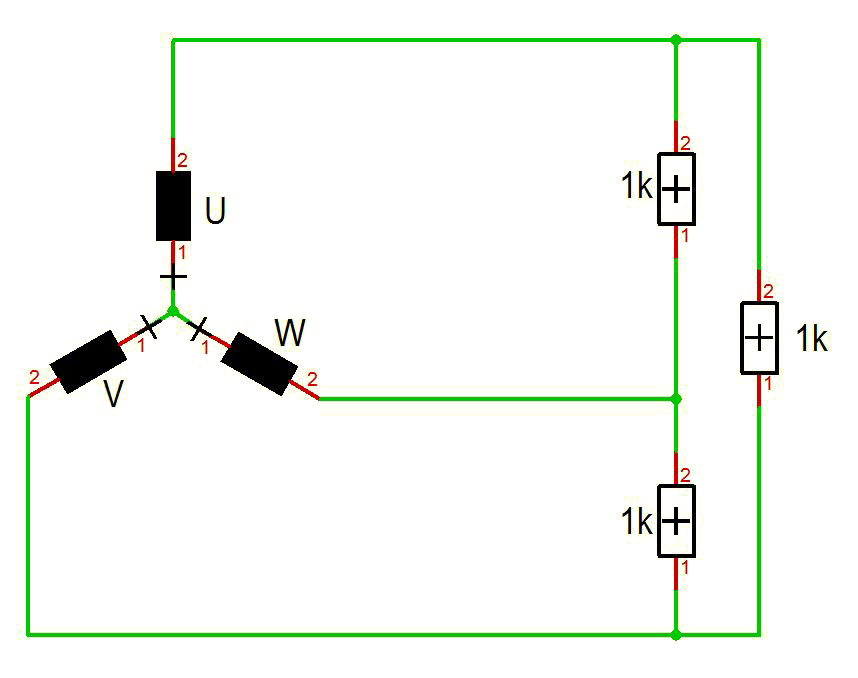
\includegraphics[height=\textheight]{Test/Messchaltung_Fremderregung}
		\caption{Messchaltung}
	\end{figure}
\end{frame}

\begin{frame}{Test und Analyse}{Analyse Spannungsmessung Fremderregung}
	\begin{figure}
		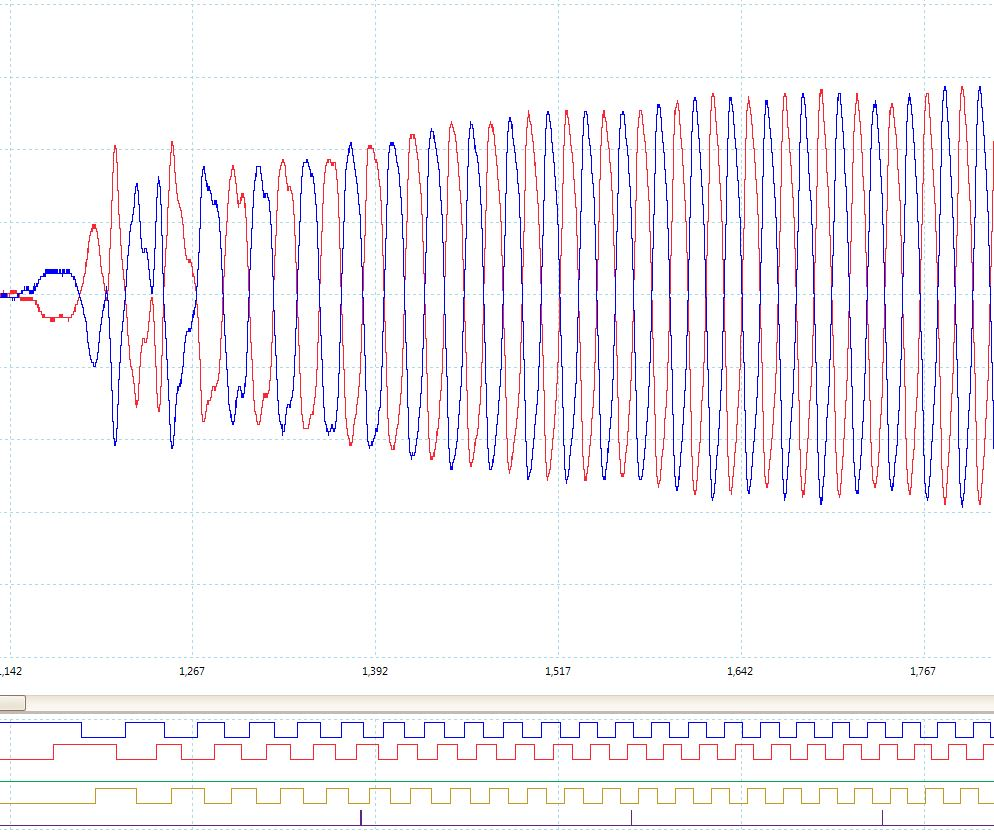
\includegraphics[height=\textheight]{Test/Spannungssignal_Messung}
	\end{figure}
\end{frame}

\begin{frame}{Test und Analyse}{Analyse Spannungsmessung Fremderregung mit Störsignalen}
	\begin{figure}
		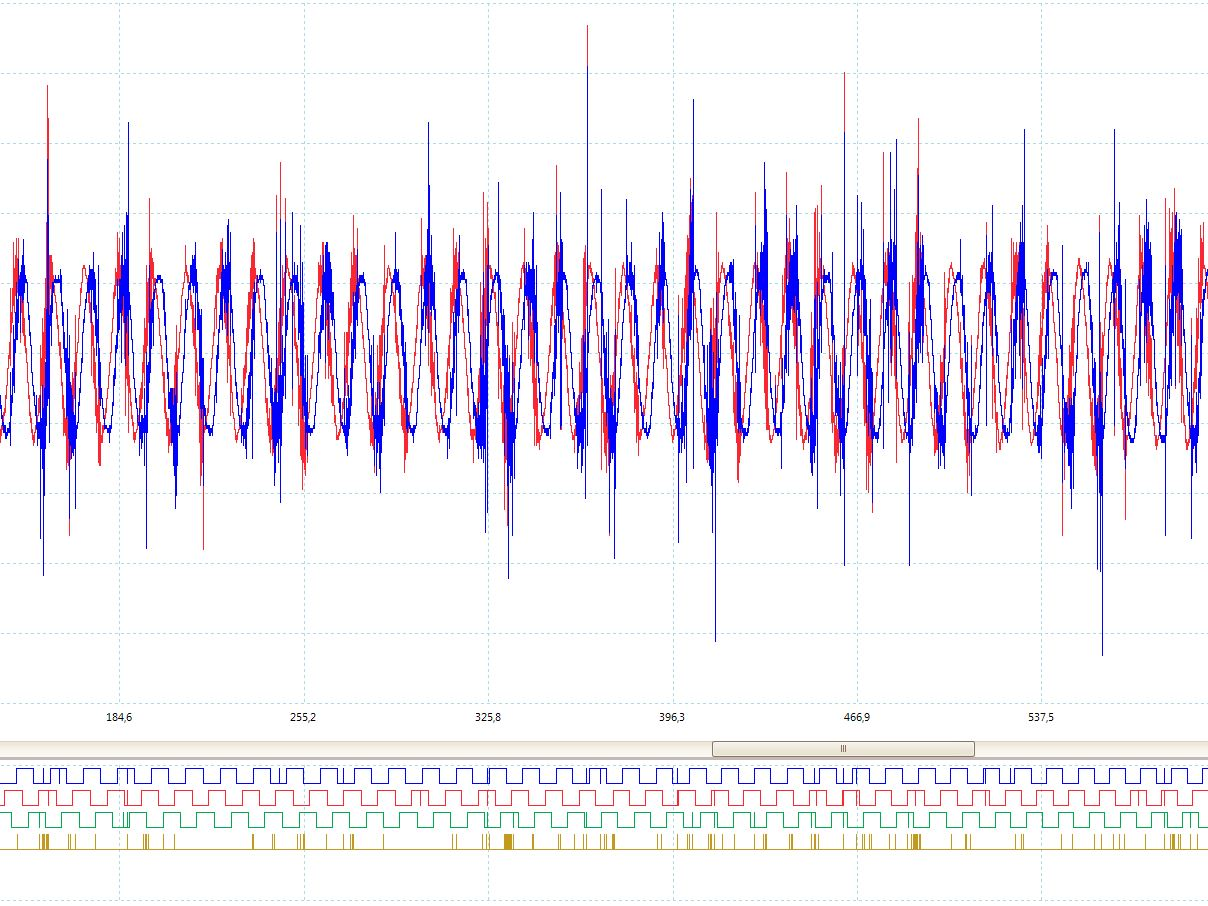
\includegraphics[width=\textwidth]{Test/Spannungssignal_Messung_mit_Fehler}
	\end{figure}
\end{frame}

\begin{frame}{Test und Analyse}{Hall-Sensoren in Verbindung mit dem XMC 4700 Relax Kit 5V}
	\begin{itemize}
		\item XMC 4700 Relax Kit 5V
		\begin{itemize}
			\item Vorbereitet für Arduino Shields (5V)
			\item Pegelwandler (5V $\leftrightarrow$ 3.3V)
			\item Störempfindlich gegenüber längeren Messleitungen ($\approx$ 20 cm)
		\end{itemize}
	\end{itemize}
\vspace{\baselineskip}
\vspace{\baselineskip}
\end{frame}

\begin{frame}{Test und Analyse}{Hall-Sensoren in Verbindung mit dem XMC 4700 Relax Kit 5V}
	\begin{figure}
		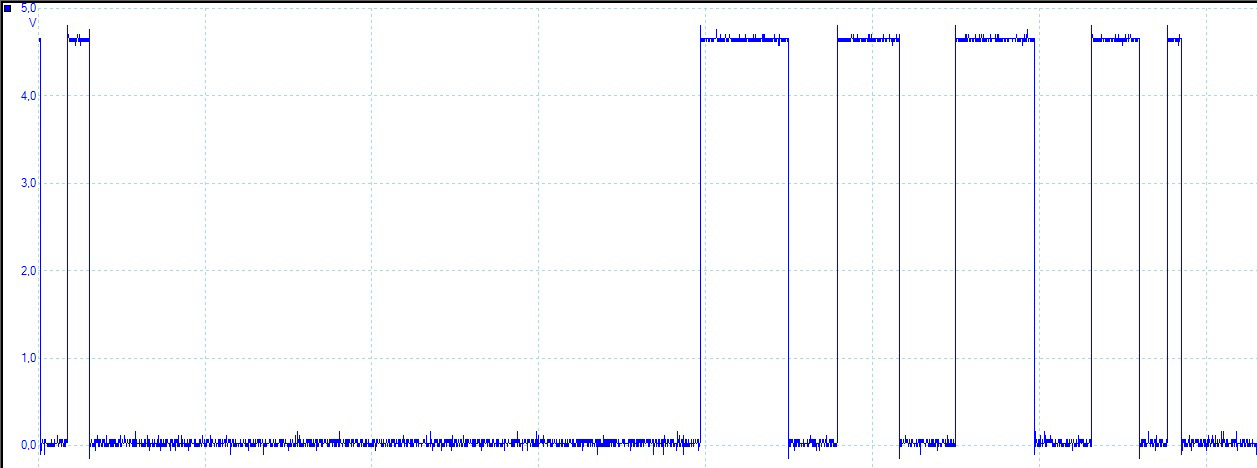
\includegraphics[height=0.4\textheight]{Test/hall_ok}
		\vspace{\baselineskip}
		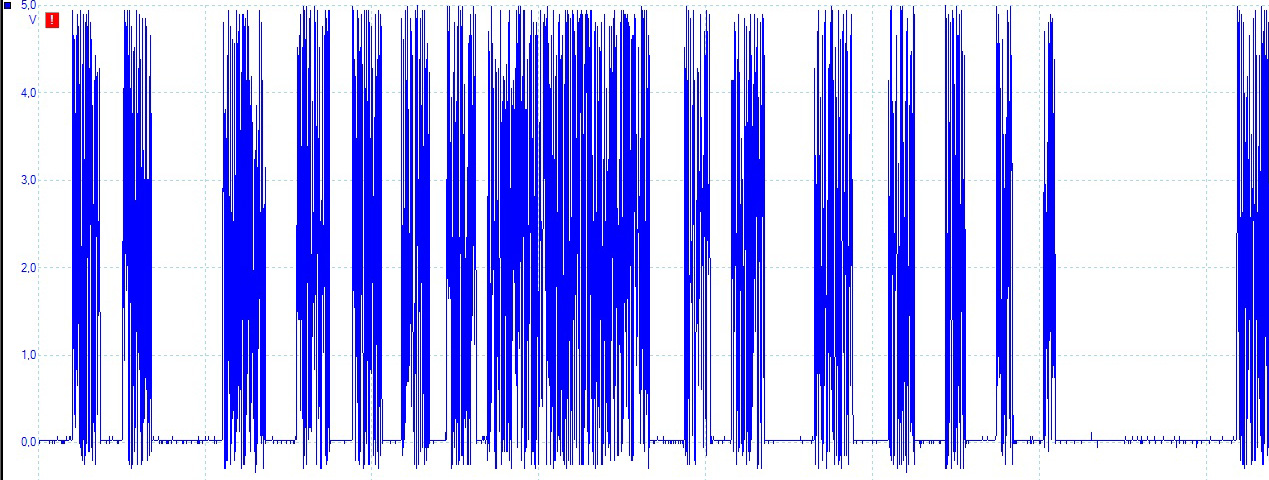
\includegraphics[height=0.4\textheight]{Test/hall_jitter_4700}
	\end{figure}
\end{frame}


\begin{frame}{Test und Analyse}{Hall-Sensoren in Verbindung mit dem XMC 4700 Relax Kit 5V}
	\begin{itemize}
		\item XMC 4700 Relax Kit 5V
		\begin{itemize}
			\item Vorbereitet für Arduino Shields (5V)
			\item Pegelwandler (5V $\leftrightarrow$ 3.3V)
			\item Störempfindlich gegenüber längeren Messleitungen ($\approx$ 20 cm)
		\end{itemize}
		\item $\rightarrow$ Messleitung verkürzen
		\item $\rightarrow$ Pegelwandler austauschen/entfernen
	\end{itemize}
\end{frame}

\begin{frame}{Test und Analyse}{Steuerung BLDC - Schaltung}
	\begin{figure}
		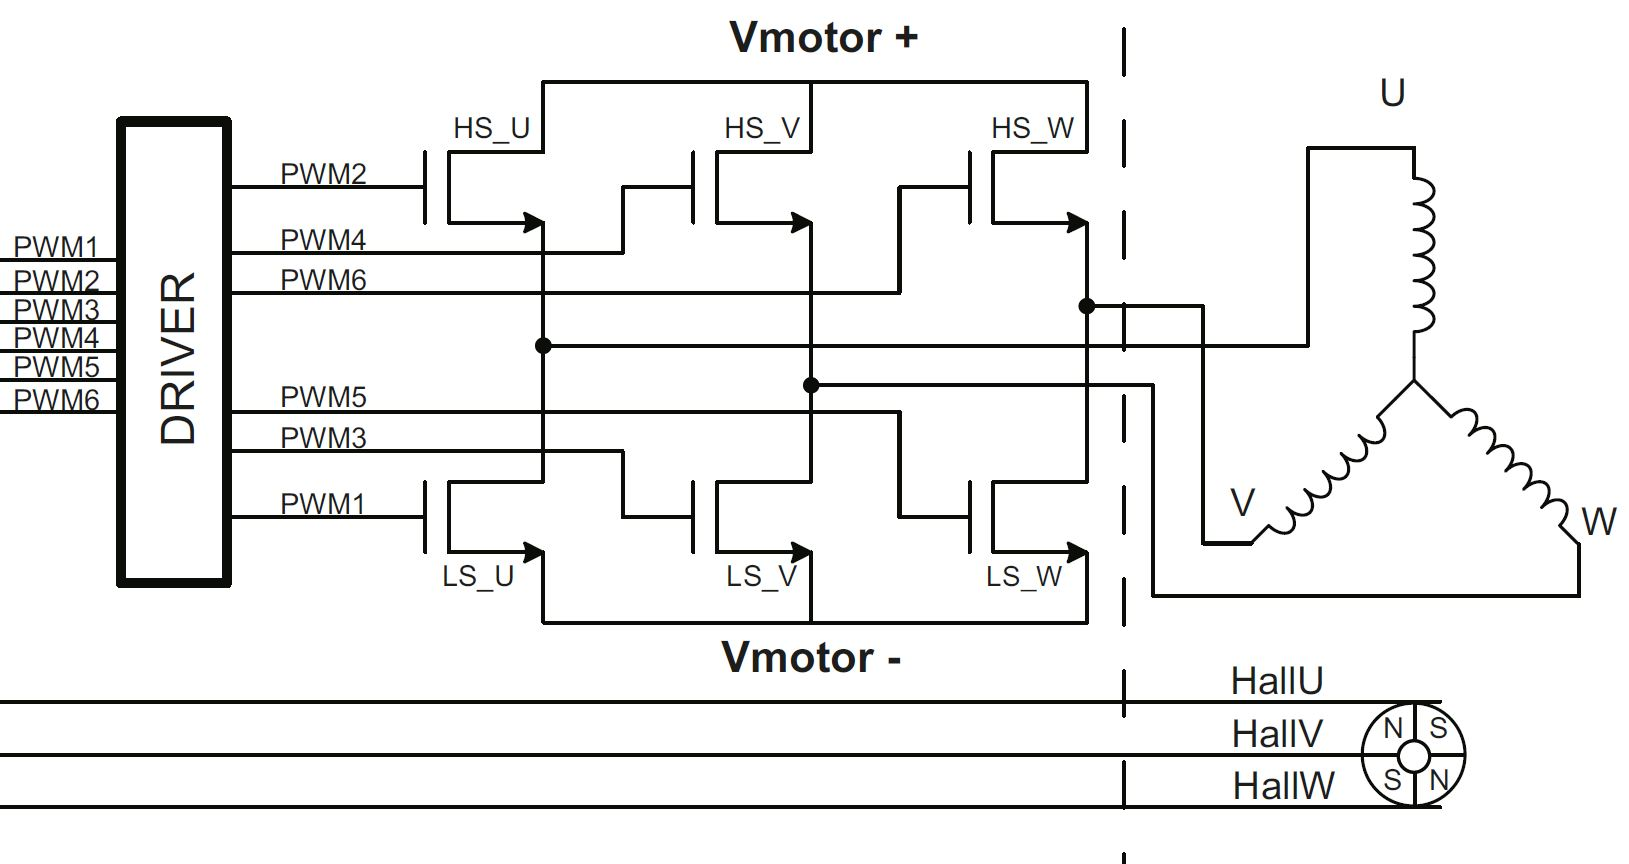
\includegraphics[width=\textwidth]{Test/Aufbau_Ansteuerung_Motor}
	\end{figure}
\end{frame}

\begin{frame}{Test und Analyse}{Steuerung BLDC - Steuersignal}
	\begin{figure}
		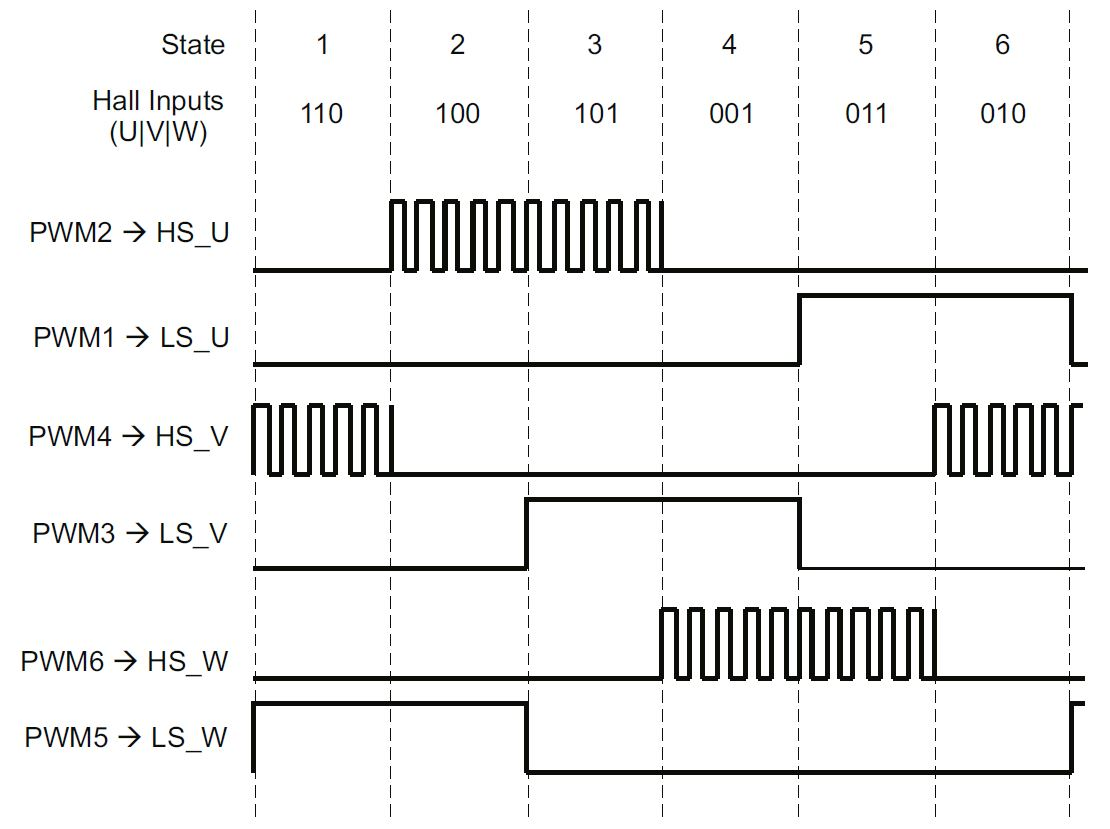
\includegraphics[height=0.8\textheight]{Test/Ansteuerung_H-Bruecke}
	\end{figure}
\end{frame}

\begin{frame}{Test und Analyse}{Steuerung BLDC - Texas Instrument}
	\begin{figure}
		\begin{itemize}
			\item Abweichende Signale
			\item Zwei Ausgänge gleichzeitig HIGH
		\end{itemize}
		\vspace{\baselineskip}
		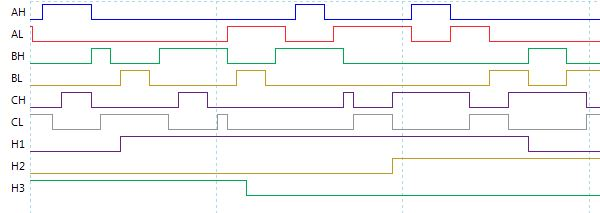
\includegraphics[width=\textwidth]{Test/Steuersignale_TI}
	\end{figure}
\end{frame}
